\documentclass[a4paper, 12pt, oneside]{scrbook}
\usepackage[hyphens,spaces,obeyspaces]{url}
\usepackage[sorting = none, backend=bibtex]{biblatex}
\usepackage[english]{babel}
\usepackage[T1]{fontenc}
\usepackage[utf8]{inputenc}
\usepackage[hidelinks]{hyperref}
\usepackage{graphicx}
\usepackage{subcaption}
\usepackage{epstopdf}
\usepackage{lmodern}
\usepackage{float}
\usepackage{acronym}
\usepackage{booktabs}
\usepackage{caption}
\usepackage{csquotes}
\usepackage{enumitem}
\usepackage{fancyhdr}
\usepackage{url}
\usepackage{listings}
\usepackage[table]{xcolor}
\usepackage{wrapfig}
\usepackage{forest}
\usepackage{tabularx}
\usepackage{colortbl}
\usepackage{booktabs}
\usepackage[onehalfspacing]{setspace}
\usepackage{amsmath}
\usepackage{threeparttable}
\usepackage[english]{cleveref}
\renewcommand*{\headfont}{\normalfont}
\renewcommand*{\multicitedelim}{\addsemicolon\space}
\renewcommand*{\headrulewidth}{0pt}
\renewcommand*{\arraystretch}{1.5}
\setlength{\parskip}{1.5ex}
\makeatletter
% define new boolean conditional switch for whether
% the abstract is being typeset
\newif\ifabstract
% redefine `\chapter` so it only starts a new page if not typesetting
% the abstract; sets abstract conditional to false after doing so
\renewcommand\chapter{\ifabstract\relax\else%
	\if@openright\cleardoublepage\else\clearpage\fi%
	\fi
	\abstractfalse%
	\thispagestyle{plain}%
	\global\@topnum\z@
	\@afterindentfalse
	\secdef\@chapter\@schapter}

% command for putting the title and name above the abstract; switches
% abstact boolean to true for next `\chapter*` command...
\newcommand{\conclusion}{
	\if@openright\cleardoublepage\else\clearpage\fi
		\begin{center}
			\textbf{\larger{Summary}}\par
			\emph{Hier kommt nach der Fertigstellung der Arbeit noch eine Zusammenfassung der Arbeit mit ein oder mehreren Sätzen hin. Hier kommt nach der Fertigstellung der Arbeit noch eine Zusammenfassung der Arbeit mit ein oder mehreren Sätzen hin. Hier kommt nach der Fertigstellung der Arbeit noch eine Zusammenfassung der Arbeit mit ein oder mehreren Sätzen hin2. }\par
		\end{center}

	\abstracttrue}
\makeatother
\lstset
{
         basicstyle=\footnotesize\ttfamily,
         numbers=left,               	% Ort der Zeilennummern
         numberstyle=\tiny,          	% Stil der Zeilennummern
%         stepnumber=2,               	% Abstand zwischen den Zeilennummern
         numbersep=5pt,              	% Abstand der Nummern zum Text
         tabsize=2,                  	% Groesse von Tabs
         extendedchars=true,
         breaklines=true,            	% Zeilen werden Umgebrochen
         keywordstyle=\color{red},
            frame=b,
 %        keywordstyle=[1]\textbf,    	% Stil der Keywords
 %        keywordstyle=[2]\textbf,
 %        keywordstyle=[3]\textbf,
 %        keywordstyle=[4]\textbf, \sqrt{\sqrt{}}
         stringstyle=\color{white}\ttfamily,
         showspaces=false,
         showtabs=false,
         xleftmargin=27pt,
         framexleftmargin=27pt,
         framexrightmargin=5pt,
         framexbottommargin=4pt,
%         backgroundcolor=\color{lightgray},
         showstringspaces=false      	% Leerzeichen in Strings anzeigen ?
}
\addbibresource{bibliography.bib}

\begin{document}
	\frontmatter
	\def\doctype{T3\_3000}
\def\title{Grafana als (alternative) Dashboardlösung für industrielle „Use Cases“}
\def\author{Rico Kursidem}
\def\supervisor{Steffen Michalowski}

\begin{titlepage}

\vspace{10mm}

\begin{center}
	
	\vspace{5mm}
	\huge \title
	
	\vspace{34pt}
	\large \doctype
		
	\vspace{30pt}	
	\small Projekt für Angewandte Informatik \\
	\large Duale Hochschule Baden-Württemberg Mosbach \\
	\small Studienpartner \\
	\large AZO GmbH \& Co. KG \\
    \vspace{35pt}
    
    
\includegraphics[height=2.5cm]{prefix/image/logo-dhbw.eps}
    
\includegraphics[height=2.5cm]{prefix/image/logo-azo.png}
	
	\vspace{40pt}	
	\small von \\
	\large \author \\
	\small betreut von \\
	\large \supervisor
\end{center}

\vspace{75pt}


\vspace{49.7pt}

\fancypagestyle{empty}{
  \fancyhf{}
  \fancyfoot[C]{\today}
}

\end{titlepage}
	%\chapter*{Abbreviation} 
\begin{acronym}
	%A
	%B
	%C
	%D
	%E
	\acro{test}{Test}
	%F
	%G
	%H
	%I
	%J
	%K
	%L
	%M
	%N
	%O
	%P
	%Q
	%R
	%S
	%T
	%U
	%V
	%W
	%X
	%Y
	%Z
\end{acronym}
	\tableofcontents
	\listoffigures
	%\listoftables
	%\lstlistoflistings
	\nocite{*}

	\mainmatter

	\pagebreak
%	\conclusion
	\chapter{Einführung}
	
	% Hinführung		- *
	% Thema 			- *
	% Problemstellung	- *
	% Relevanz			- *
	% Ziel 				- *
	
	\noindent Daten und der Einsatz von ihnen im industriellen Umfeld ist nicht mehr wegzudenken. Die Fähigkeit, Daten visuell darzustellen und so dem Administrator des Systems Mustererkennung möglich zu machen, ist essenziell zur Entscheidungsfindung. Auch das Monitoring von Live-Daten ist wichtig. 
	Eine Möglichkeit zur Visualisierung von Daten sind Grafen, Tabellen und andere grafische Darstellungen. Diese Grafen müssen daraufhin in Dashboards angezeigt und geordnet werden, um dem menschlichen Nutzer das beste Verständnis der Daten zu versichern.
	
	\noindent Eine eigene Lösung für diese Aufgabe zu implementieren ist umfangreich und führt oftmals zu nicht zufriedenstellenden Ergebnissen. Deshalb viel der Blick auf die Open-Source Technologie Grafana, welche das einfache und schnelle einbinden von Datenquellen und Visualisierung von Daten ermöglicht. Grafana soll bei AZO in ein Projekt eingebunden werden und muss deshalb Anforderungen erfüllen. Das Ziel dieser Arbeit ist es die Anforderungen zu betrachten, zu beschreiben und eine erste Informationsbasis zu schaffen, auf der entschieden werden kann, ob Grafana sich als Visualisierungswerkzeug für AZO eignet.
		
	\chapter{Technische Grundlagen}
	
		\section{Docker}
			\noindent Docker ist eine Open Source Virtualisierungssoftware mit welcher die Ausführung von Applikationen in Containern möglich ist. Jede Anwendung bekommt einen eigenen Container mit individueller Umgebung und läuft dann, parallel zu anderen Containern, auf demselben Host. Docker Container sind leichtgewichtiger da sie sich, anders als VMs, ein gemeinsames Betriebssystem teilen. Außerdem werden redundante Dependencies von einzelnen Containern nicht dupliziert, sondern als gemeinsame Ressource abgespeichert. Ein anderer Vorteil von Docker Containern ist der einfache Transport. In einem Image werden hierfür alle nötigen Informationen abgespeichert. Die Dependencies und der Code der Anwendung. Dann muss nur das Image übertragen, ein Container daraus erstellt und auf einem beliebigen System mit der Docker Engine gestartet werden und die Applikation läuft.
			
			\noindent Das Testsystem, auf welchem diese Arbeit basiert, nutzt Docker zur Bereitstellung zahlreicher Dienste. Wichtig für diese Arbeit sind der Grafana, Node-Red und Datenbank Container.
			
		\section{ACAS}
			\noindent ACAS ist eine intern bei AZO entwickelte Automatisierungsplattform. Sie soll eine Schnittstelle zwischen Bediener und Anlage sein. Dabei sollen diverse Aufgaben wie Virtualisierung, Fehlererkennung und Monitoring erfüllt werden. Grafana soll als Monitoring Tool eingesetzt werden um Anlagen im Betrieb zu überwachen und Fehlerursachen frühzeitig zu erkennen um Schäden zu minimieren.
			
		\section{Grafana}
			\noindent Grafana ist eine Open Source Software, mit der dynamische Dashboards zur Überwachung und Auswerten von Daten angefertigt werden können. Grafana bietet hierzu eine zugängliche und simple Benutzeroberfläche zur Erstellung von einzelnen Diagrammen die Panels genannt werden. Grafana bietet State of the Art Funktionen wie da Verschieben und individualisieren von Oberflächen und zahlreiche Datenquellen, sodass es eine solide Lösung für Monitoring, Fehlererkennung und Analyse darstellt.
			
			\noindent Grafana läuft in einem Docker Stack zusammen mit einem Node-Red und Datenbank Container. Der Container verwendet die Version 9.3.0 von Grafana.
	
	\chapter{Funktionsanalyse}
	 
		\section{Einbinden von Datenquellen}
	 
			\noindent Grafana soll als Visualisierungswerkzeug in ACAS, dem bereits bestehenden System, integriert werden und die bereits bestehenden Datenquellen einbinden. Die Anforderungen an das System beinhalten die Anzeige von Daten aus einer Microsoft SQL Datenbank und Sensordaten, welche von einer SPS geliefert werden. Das Integrieren einer MSQL Datenbank ist bereits nativ von Grafana unterstützt. Zunächst muss die Datenbank in Grafana als Datenquelle eingebunden werden. Wenn alle Verbindungs- und Authentifizierungsinformationen konfiguriert sind, kann die datenquelle in den Paneleinstellungen verwendet werden. In Abbildung \ref{fig:mssql_ein} ist eine exemplarische Anfrage an  den SQL Server abgebildet, bei dem die Anzahl der unterschiedlichen Wiegefehler ausgegeben wird. Die Tabelle, die durch die Anfrage zurückgegeben wird, kann dann in verschiedensten Diagrammen visualisiert werden.
	 	
	 \begin{figure} [H]
	 	\centering
	 	\resizebox{\linewidth} {!} {
	 		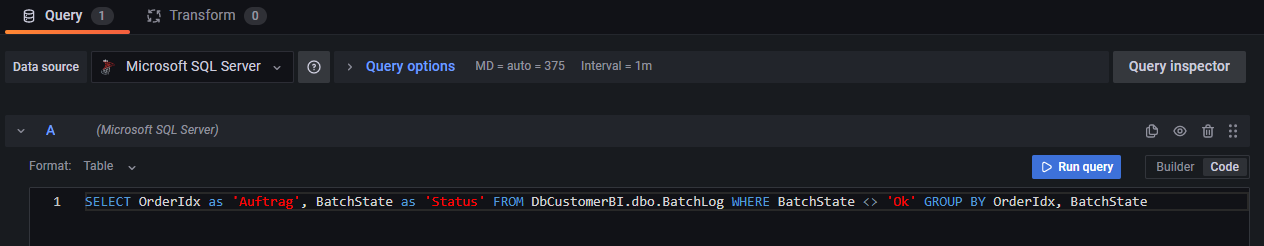
\includegraphics{res/mssql_einbinden.png}
	 		
	 	}
	 	\caption{Einbinden von MSSQL Datenbanken}
	 	\label{fig:mssql_ein}
	 \end{figure}
 	
 		\noindent Um Daten aus einer SPS auf einem Grafanadashboard anzeigen zu lassen, müssen die Daten zunächst in eine Datenbank geschrieben und dann nach Grafana exportiert werden, da Grafana keine native Möglichkeit besitzt, MQTT Daten einzulesen. Um den Datentransport zu machen, wird ein Node-Red Server verwendet. In Abbildung \ref{fig:nodered} ist der Node-Red-Flow abgebildet. Zunächst werden die Daten aus der SPS gelesen. Dies wird möglich durch eine native S7-Kopplung die Daten aus einer SPS in Node-Red portiert. Im Anschluss werden die Daten über einen MQTT Broker in eine InfluxDB geschrieben die in Grafana als Datenquelle eingebunden werden kann, wie die Microsoft SQL DB bevor.
 		
 		\begin{figure} [H]
 			\centering
 			\resizebox{\linewidth} {!} {
 				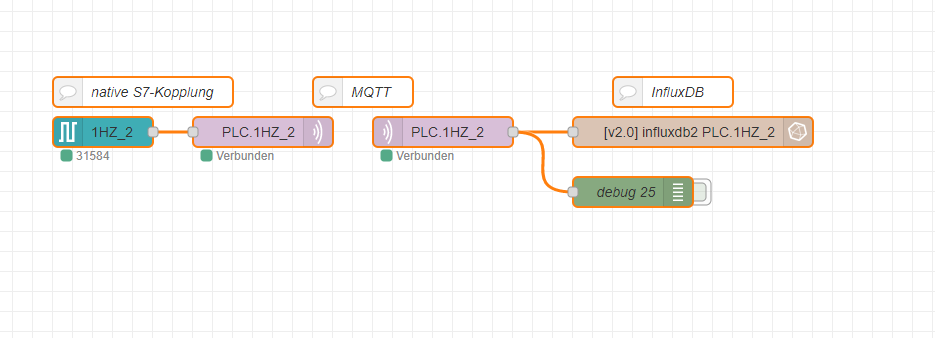
\includegraphics{res/nodered.png}
 				
 			}
 			\caption{Node-Red Flow mit Rückgabe einer JSON}
 			\label{fig:nodered}
 		\end{figure}
 	
	 	% \noindent Um JSON Daten in Grafan verarbeiten zu können muss ein Plugin integriert werden. Hierbei fiel die Entscheidung auf das "Infinity" Plugin von Sriramajeyam Sugumaran da es neben der Integration von JSON Daten auch XML, CSV und weitere Datenformate unterstützt und regelmäßige Updates bekommt. In den Data Sourcen Einstellungen können weitere Einstellungen vorgenommen werden, die für den in dieser Arbeit nicht von Nöten sind. Wird die Data Source in einem Panel dann ausgewählt, muss die Adresse des API Aufrufs und optionale Übergabe Parameter eingetragen werden. Bei jeder Aktualisierung wird der API Abfrage getätigt und die Daten visualisiert. 
	 	
	 	% \noindent Um die Sensordaten ansehnlich zu präsentiere, können Transformationen genutzt werden. Im Transformationen Reiter kann die Funktion "Rows from Fields" wie in Abbildung \ref{fig:transformation} ausgewählt werden, welche die Werte gewisser Spalten zu Konfigurationswerten übernimmt. 
	 	
	 	%\begin{figure} [H]
	 	%	\centering
	 	%	\resizebox{75mm} {!} {
	 	%		
	 	%	}
	 	%	\caption{Transformation der Sensordaten}
	 	%	\label{fig:transformation}
	 	%\end{figure}
	 	
	 	\noindent Um Daten zur Darstellung der Daten über werte aus einer Datenbank zu manipulieren können Transformationen verwendet werden. Um Schwellenwerte zu laden um beispielsweise kritische Sensorwerte in einer anderen Farbe darzustellen können Thresholds festgelegt werden. Werden diese in Grafana statisch erstellt, können multiple untere Schwellenwerte und Bereiche mit verschiedenen Farben erstellt werden. Mit Daten aus einer Anfrage kann bis jetzt mit der "Config from Rows" oder "Rows from Fields" nur ein Schwellenwert festgelegt werden. Alledings befinden sich diese Funktionen in einem Beta Stadium und eine erweiterte Funktionalität ist zu erwarten. \cite{GrafanaLabs:Thresholds}
	 	
	 	% TODO: Transformation und Thresholds - weiter? 
 		
	 \section{Interaktion zwischen Grafen}
	 	
	 	\subsection{Filterungen durch Variablen}
	 	
	 	\noindent Grafana bietet dashboardweite Variablen, welche zuvor festgelegte Werte annehmen können. Diese Werte sind entweder manuell eingetragen oder aus Datenquellen ausgelesen. In den Dashboardeinstellungen können Variablen angelegt und ihre Wertauswahl konfiguriert werden. Jede Variable kann ganz oben auf einem Dashboard angezeigt und dort anhand eines Drop-Down-Menüs gesetzt werden. 
	 	
	 	\noindent Um die erstellten variablen in beispielsweise SQL Anfragen zu verwenden, kann ein Dollarzeichen und der Variablenname eingegeben werden (Beispiel: \texttt{\$variableName})\cite{GrafanaLabs:Variables}. Soll die Variable innerhalb eines durchgehenden Strings verwendet werden, können geschweifte Klammern genutzt werden, um die Variable vom Text zu trennen (Beispiel: \texttt{\$\{variableName\}})\cite{GrafanaLabs:Variables}. Eine Variable kann auch mit einer Auswahlfunktion generiert werden, um mehrere Parameter in dieser Variable zu speichern. So können die Daten mehrerer Sensoren oder Anlagen gezeigt werden. In einer SQL Abfrage können diese mit dem IN Schlüsselwort genutzt werden (Beispiel: \$\{variableName\})\cite{GrafanaLabs:Variables}. Außerdem kann ein Panel oder eine ganze Row als "Repeating by variable" konfiguriert werden, um einmal pro Auswahlparameter der Variable erstellt zu werden. Sind beispielsweise mehrere Sensoren ausgewählt, wird für jeden Sensor ein Panel oder eine Row erstellt.
	  	
		\subsection{Links}
		 
		\noindent Bei Verlinkungen werden zwischen drei verschiedenen Links unterschieden. Dashboard Links, Panel Links und Data Links. Dashboard Links können in den Einstellungen des Dashboards erstellt werden und erscheinen dann in der oberen rechten Ecke des Dashboards. Um einen Link des Zieldashboards zu erstellen, muss auf das Teilen Symbol 
\includegraphics{res/teilensymbol.png} neben dem Namen geklickt werden und der Link kopiert werden. Panel Links sind Verlinkungen, welche an einem Panel angehangen sind. Sie erscheinen in der oberen linken Ecke eines Panels. Data Links können innerhalb eines Panels angelegt werden und können auf Informationen zugreifen, welche Daten in der Grafik gedrückt wurden. 
		
		\noindent Um Informationen von einem Dashboard zum nächsten zu übermitteln können Dashboardweite Variablen verwendet werden. In Tabelle \ref{tab:links} ist der Syntax der verschiedenen Übergabemöglichkeiten aufgeführt. Es können konstante Werte, Dashboard Variablen oder Datenpunkte übergeben werden, wobei bei der Eingabe von einem Dollarzeichen Grafana bereits alle möglichen Felder in einem Drop-Down-Menü vorschlägt und bei Auswahl den korrekten Syntax einträgt. \texttt{varName} ist dabei die Variable des Zieldashboards welche den gewählten wert annehmen soll.
			 
		\begin{figure} [H]
			\centering
			\resizebox{\linewidth} {!} {
	 		\begin{tabular}[h]{|l|c|}
	 			\hline
	 			Variable & Übergabe im Link \\
	 			\hline
	 			Konstante & \texttt{var-varName=value} \\
	 			\hline
	 			Variable &  \texttt{var-varName=\${DashBoardVar}} \\
	 			\hline
	 			Datenpunkt &  \texttt{var-varNname=\${\_\_data.fields.FieldName}} \\
	 			\hline
	 			Zeitintervall als url &  \texttt{\${\_\_url\_time\_range}} \\
	 			Intervall Start& \texttt{\$\_\_timeTo()} \\
	 			Intervall Ende& \texttt{\$\_\_timeFrom()} \\
	 			\hline
	 		\end{tabular}
		}
		 		
	 	\caption{Übergabeparameter in Links}
	 	\label{tab:links}
	\end{figure}
		 
	\noindent es kann auch auf das selbe Dashboard verlinkt und die Variablen gesetzt werden, wodurch die Manipulation von Panelen über den Klick auf ein anderes Panel ermöglicht wird.
			 
			 
	\subsection{Annotationen}
			 
	\noindent Annotationen können genutzt werden um bestimmte Ereignisse aus Zeitreihen auf dem gesamten Dashboard hervorzuheben. Diese Ereignisse können durch eine Datenquelle als Zeitabhängige Datenpunkte eingelesen werden. Sie werden dann auf jedem Zeitreihen Grafen markiert wie in Abbildung \ref{fig:annotations} die Fehlermeldungen in rot.
		 
	\begin{figure} [H]
	 	\centering
	 	\resizebox{\linewidth} {!} {
	 		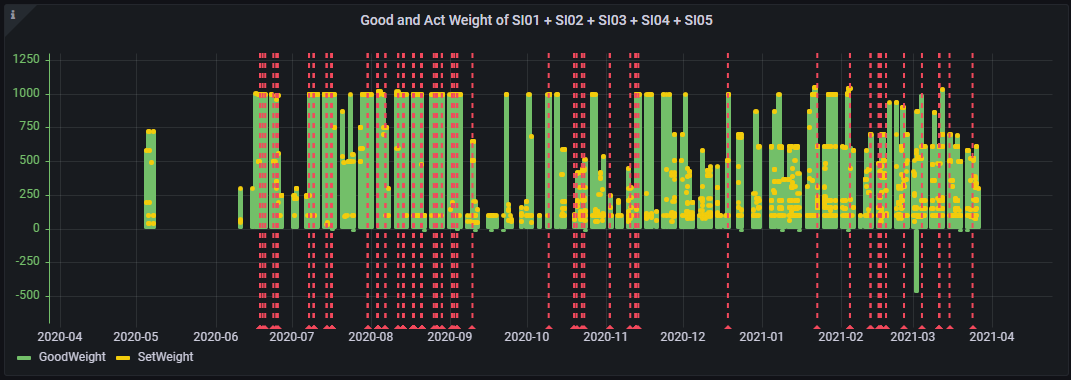
\includegraphics{res/annotaitons.png}
	 		
	 	}
	 	\caption{Annotationen in einer Zeitreihe}
	 	\label{fig:annotations}
	 \end{figure}
	 
	 \section{Berechtigungen und Rollenkonzepte}
	 
	 \noindent Grafana stellt drei Rollen zu Verfügung. Admin, Editor und Viewer. Viewer haben nur die Möglichkeit, Dashboards zu besuchen während Editoren sie bearbeiten können. Administratoren haben darüber hinaus Berechtigungen zur Serverweiten Einstellungen wie Nutzereinstellungen, Plugins und Datenquellen. 
	 	
	\noindent Jeder Nutzer hat eine default Rolle, welche Serverweit gilt, jedoch können die Berechtigungen auch von Dashboard zu Dashboard überschrieben werden um Rechte individuell festzulegen. Um Rollenkonzepte anzulegen können Nutzer zu Teams zugewiesen werden welche auch auf jedem Dashboard Rollen zugeteilt bekommen können. 
	 	
	\section{Erscheinungsbild und Design}
	 
	\noindent Grafana erlaubt die Auswahl zwischen einem Dark und Light Theme, allerdings gibt es keine offiziell unterstützte Funktion, Hintergrund, Schrittfarbe und weitere Konfigurationen zu verändern. Es gibt die Möglichkeit die Veränderungen direkt in den TypeScript-Dateien zu verändern. Das bringt jedoch mit sich. Zum einen könnte nach jedem Update ein Veränderung der Struktur dazu führen, das die Änderungen der Dateien unnötig werden. Zum anderen müssen nach jedem Update alle änderungen neu eingespeilt werden. Ds größte Problem ist jedoch, das der Grafana Container von Lokalen Quellen erstellt werden muss, wodurch die Grafana Anwendung nicht immer auf dem neusten stand bleibt.
	
	\noindent Die Änderungen des Erscheinungsbildes kann jedoch mit dem "Boom Theme" angepasst werden. Allerdings sind diese Anpassungen nur für ein Dashboard einstellbar und können von Endnutzern ebenfalls abgeändert werden. Aufgrund dessen ist die Anpassung von Grafana an den Firmeninternen Designstiel nicht möglich.
	
	\chapter{Fazit}
		
	\noindent Grafana verspricht eine nutzerfreundliche und schnelle Erstellung von Dashboards zur Visualisierung von industriellen Daten. Dieses Versprechen wird durch die zahlreichen Datenquellen, Visalisierungsforemen und Erstellungsmenüs gehalten. Es erfüllt alle Anforderungen für die Implementation der vorhandenen Datenquellen und enthält genug Wege zur dynamische Interaktion von einzelnen Paneelen. Außerdem ist ein Rollenkonzept bereits mitgeliefert. Das Design der Oberfläche lässt sich nicht in die bereits bestehende Erscheinungsbild von ACAS integrieren.

	%TODO: Abschlusssatz
	
	\frontmatter
	\printbibliography

\end{document}
